\section{RIMA1 and RIMA2: Conditianal Assessment Robotic Tools for Sewer Pipes}

\label{sec:industry}

\textbf{Brief: } RIMA1 [~\ref{fig:rima1}] and RIMA2 [~\ref{fig:rima2}] are two robotic tools developed by the UTS Robotics Institute in collaboration with Sydney Water. They are designed to conditially assess the pipe walls of sewer 
pipes using Pulse Eddy Current (PEC) Sensors. Both robots operate in the ROS1 framework and are equipped with various sensors and cameras such as IMU and RGB-D cameras. Both robots communicate with the base station using VDSL via a 
kevlar braided cable. The subsections will go over more specific tasks I did on RIMA1 and RIMA2 meaning it will excluide things such as general maintenance and repair which was definitely done given these robtots are prototypes.

\begin{figure*}[htbp]
    \centering
    \begin{minipage}[t]{0.48\textwidth}
        \centering
        \includegraphics[width=\textwidth]{images/rima1/RIMA1_Physical_Weight_Detatched.jpg}
        \caption{RIMA1}
        \label{fig:rima1}
    \end{minipage}
    \hfill
    \begin{minipage}[t]{0.48\textwidth}
        \centering
        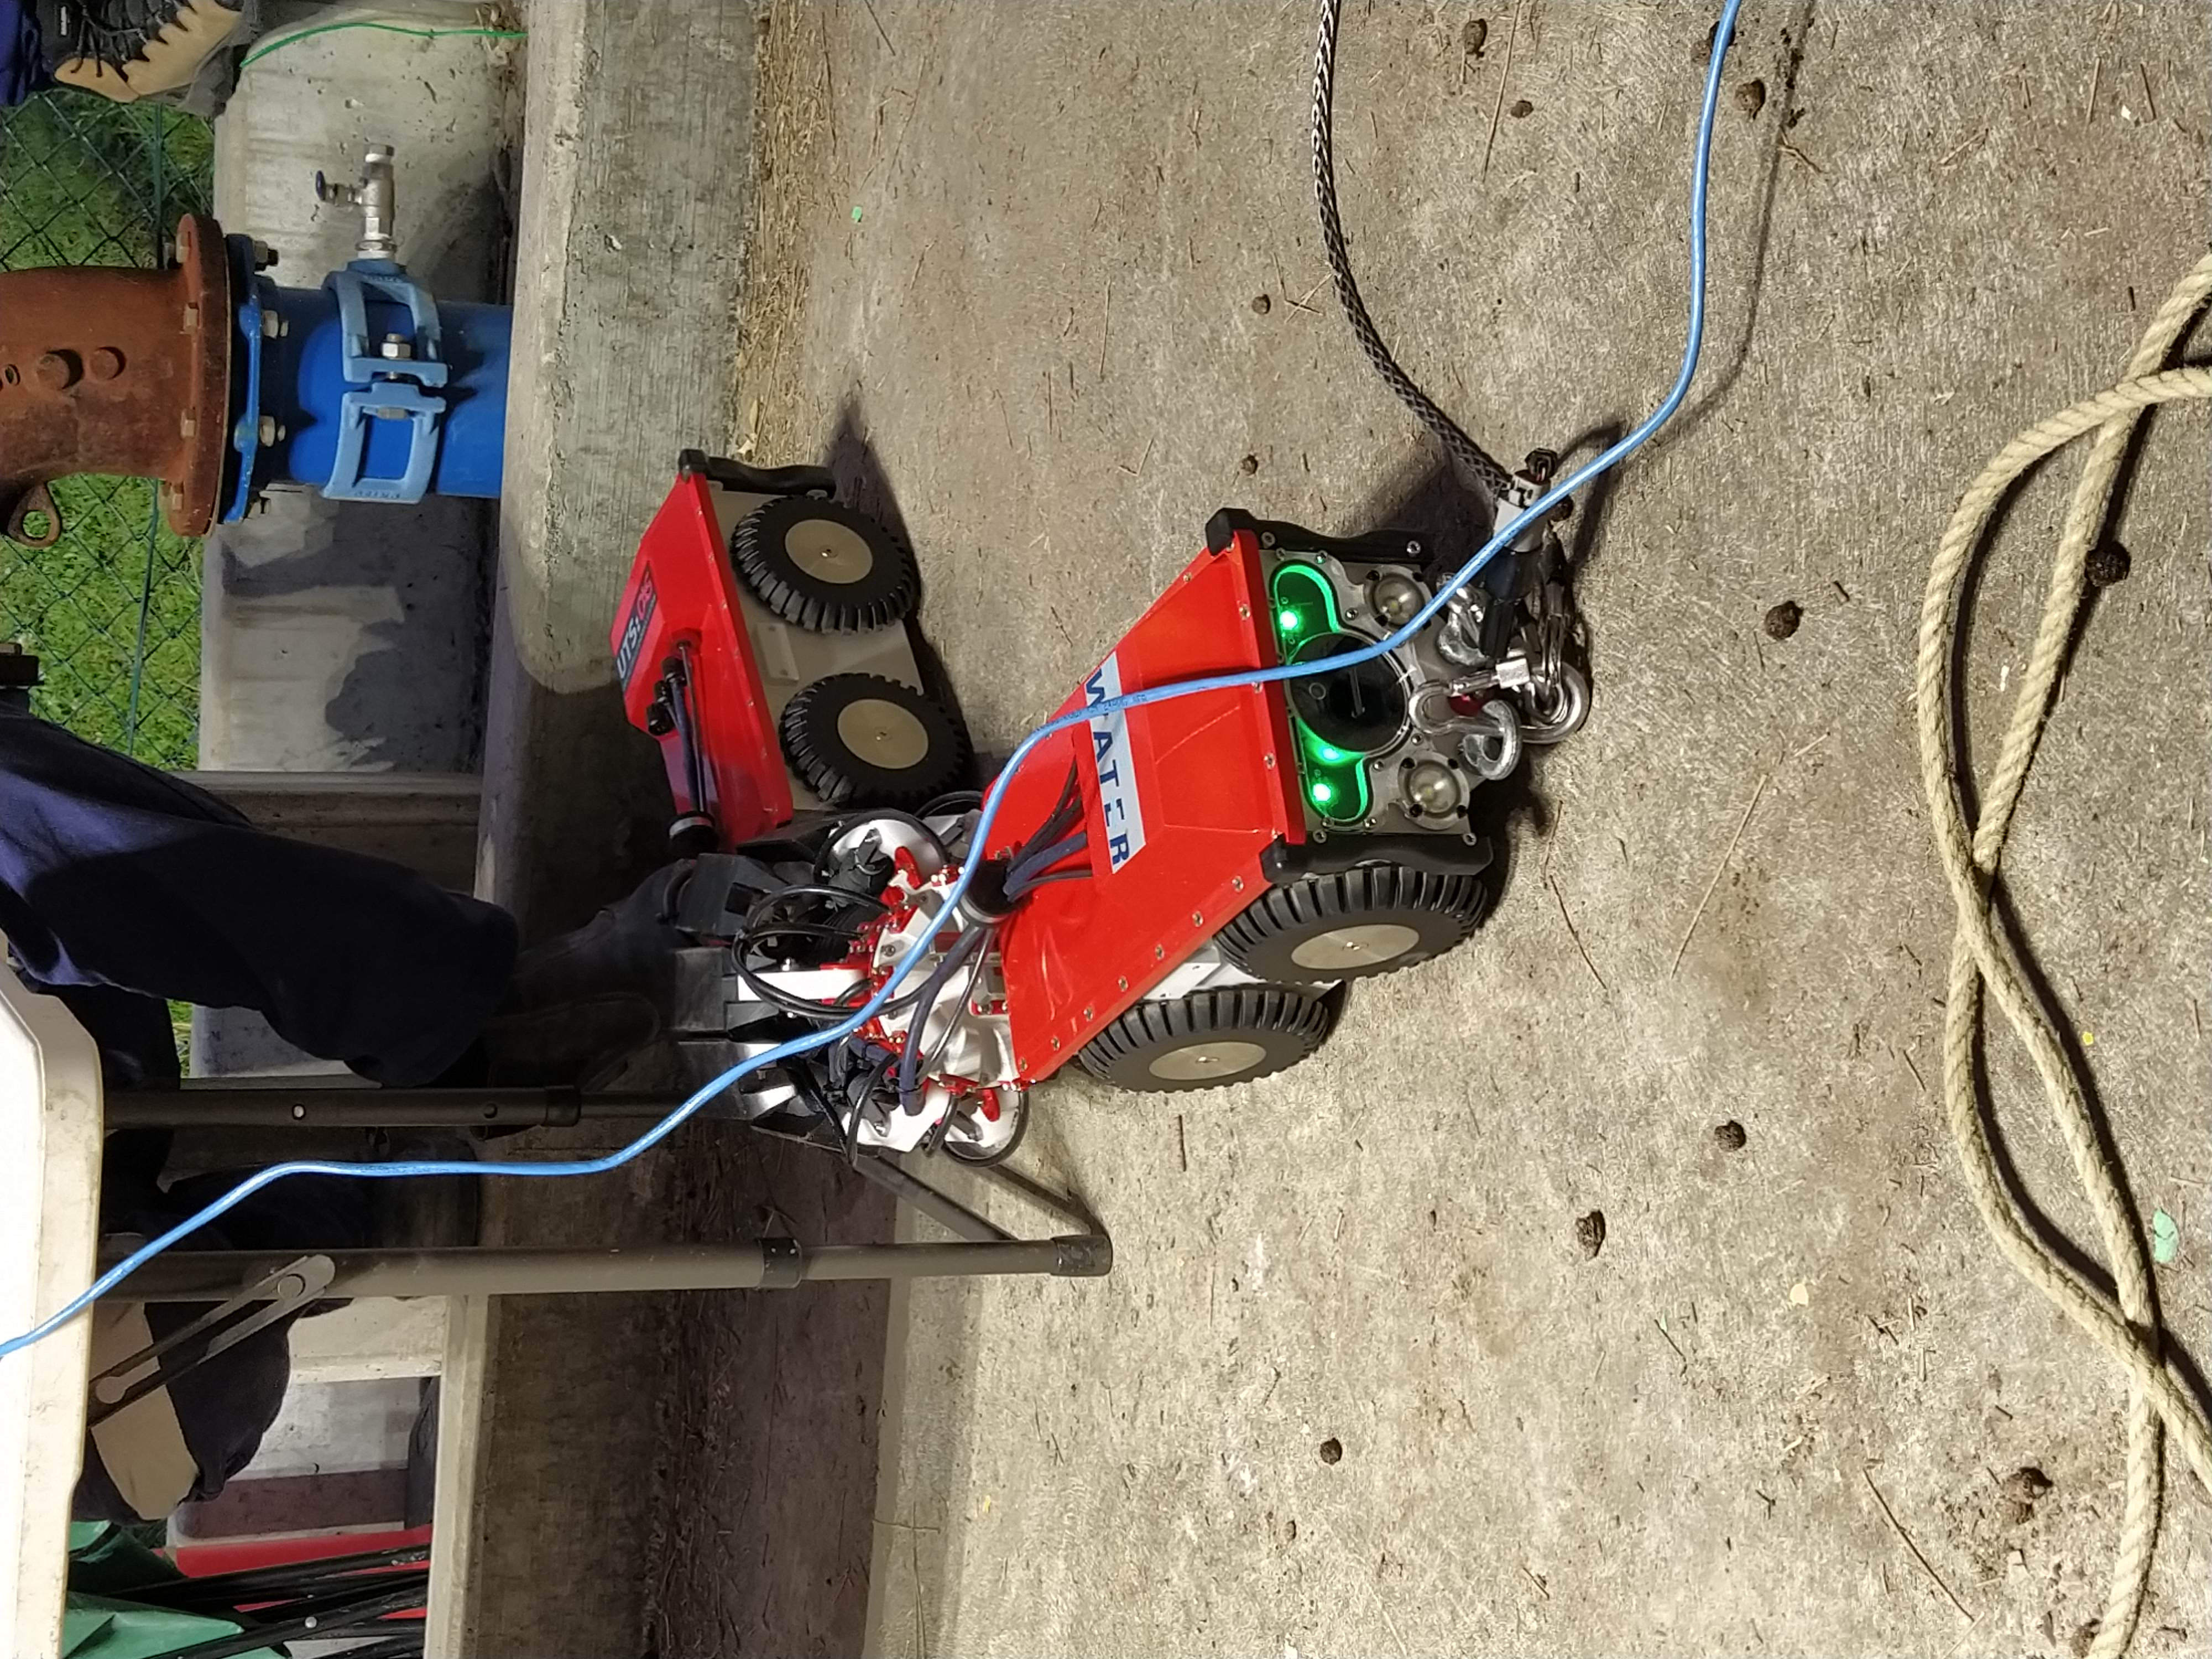
\includegraphics[angle=90, width=\textwidth]{images/rima2/RIMA2_Physical.png}
        \caption{RIMA2}
        \label{fig:rima2}
    \end{minipage}
\end{figure*}

% Tether Protetiion Section
\newpage
\subsection{Mechanical Work}

\textbf{Utilities for RIMA1 and RIMA2 Field Trials:} I designed a number of utilities to assist with field trial deployments to prevent damage to equipment and site. Using solidworks I designed
tether protection for flangless and flanged pipes [~\ref{fig:tethproc}] which were later manufactured to be used in deployments. The tether protection units are designed with the following intent:

\begin{itemize}
    \item Ease of use for Sydney Water personnel
    \item Prevent damage to the tether and pipe wall at entrance where edge is sharp
    \item Adjustability for different pipe diameters (250mm to 750mm)
    \item Stainless steel for Chemical and Weather resitance and durability
    \item Simple lock-pin mechanism to ensure ease of use when wearing gloves
    \item Teflon block with internal radius matched to the bend radius of tether cable connected from base station to the robot
    \item Simple, low cost design
\end{itemize}

\imgpairin{utility/flangless_tether_protection.JPG}{Flangless Tether Protection}{utility/tether_protection_flanged.JPG}{Flanged tether protection}{Tether Protection}{tethproc}{90}{270}

% Deployment Cradle Section
\newpage

The next utility I designed was a debloyment cradle for RIMA2 [~\ref{fig:jdm}]. Often, due to safety constraints only one person is allowed into the sewer pit. This does not favour the handling of RIMA2 which is a 3-body 
system best carried and inserted into pipes safely by two people. After an incident in a previous deployment before I started where RIMA2 was dropped, I was assigned with designing a cradle. The advantage 
of the cradle to safely lower and deploy RIMA2. The final deisgn has the following features:

\begin{itemize}
    \item Can be lowered using block-and-chain or cranes (varies with resource availability on site)
    \item Lightweight to ensure weight requirements are met as per agreement with Sydney Water
    \item Simple, intuitive locking mechanisms to ensure ease of use for Sydney Water personnel
    \item Custom flange design to adapt to various flanged pipe diameters (250mm to 450mm) if additional support is required
\end{itemize}

\imgpairin{utility/jdm.jpg}{RIMA2 Cradle in lab}{utility/jdm_in_use.jpg}{Cradle in use on field trial}{RIMA2 Cradle}{jdm}{0}{270}

% Rollover-Assist RIMA1
\newpage
\textbf{RIMA1 Rollover Assist:} I designed a set of rollover assist devices for RIMA1 after an incident in one of the first trial runs with Sydney Water having full control in our robot when unfortuntaely
a software bug caused the robot to drive autonomously up the pipe wall causing in to invert. The aim of the rollover assist is to assist in manually having to pull the robot out the pipe when it inverts, as 
using mchinery to dig up the robot can be costly, time-consuming and potentially impossible depending on location.The inital inspiration [~\ref{fig:rp}] actually came from when I pulled apart my skateboard and attached it to RIMA1.
The final design [~\ref{fig:fdra}] after a few iterations is quite different from this and is simply a modification of the Sensor Pad on the sensor head with a custom bracket that could be fitted to RIMA1 with a simple modification to the handles.  

\imginin{rima1/rollover_prototype.jpg}{Rollover Prototype}{rp}{0.29}
\imgpairin{rima1/rollover_rear.jpg}{Rollover Assist Rear View}{rima1/rollover_side.jpg}{Rollover Side View}{Final Design Rollover Assist}{fdra}{270}{0}

\subsection{Electrical Work}

% RIMA1 System Board Instalation
\textbf{RIMA1 System Board Installation:}

% RIMA2 New PEC Board Test Rig
\newpage
\textbf{RIMA2 New PEC Board Test Rig:}

% RIMA2 New PEC Board Installation
\newpage
\textbf{RIMA2 New PEC Board Installation:}


% RIMA2 Debugging
\newpage
\textbf{RIMA2 Electrical Debugging:}
\newpage
\subsection{Software Work}

% Give a brief software overview
\textbf{Software Brief: }
RIMA1 and RIMA2 ran off the ROS1 Melodic framework. They utilised custom messages and customised ROS packages to function. All code for the robot was written in C++ and analysis scripts used for PEC are written
in Python. Unfortunately the codebases for these robots cannot be shared as it is property of UTS and Sydney Water. The robots processes and GUI's are all run/launched ushing shell scripts in the linux CL.

% New RIMA1 system board software update
\vspace{\baselineskip}
\textbf{RIMA1 System Board Software Update: }
The new system board required some minor software updates. This primarily consisted of changes to message data types and names. This change also required small modification to RIMA1's core.cpp file which was resposible 
for ROS handling (i.e. setting up subscribers, publishers, etc.). 

% RIMA1 GUI Update
\vspace{\baselineskip}
\textbf{RIMA1 GUI Update: }
The old GUI of RIMA was outdated and not greatly designed and doing something simple such as turning required going into settings and modifying rotation setpoints which is clearly not ideal or user friendly. I updated
the GUI [~\ref{fig:r1gui}] to have more intuitive control, I also installed rear cameras at the time for rear view and visual view of the sensor to have a better cue of full expansion rather than basing it off the current reading. Basic 
IMU visualisation was also added to the GUI to allow for better understanding of the robot's orientation in the pipe. The GUI was written in C++ using Qt Designer.

\begin{figure*}[htbp]
    \centering
    \subfloat[Old RIMA1 interface]{
        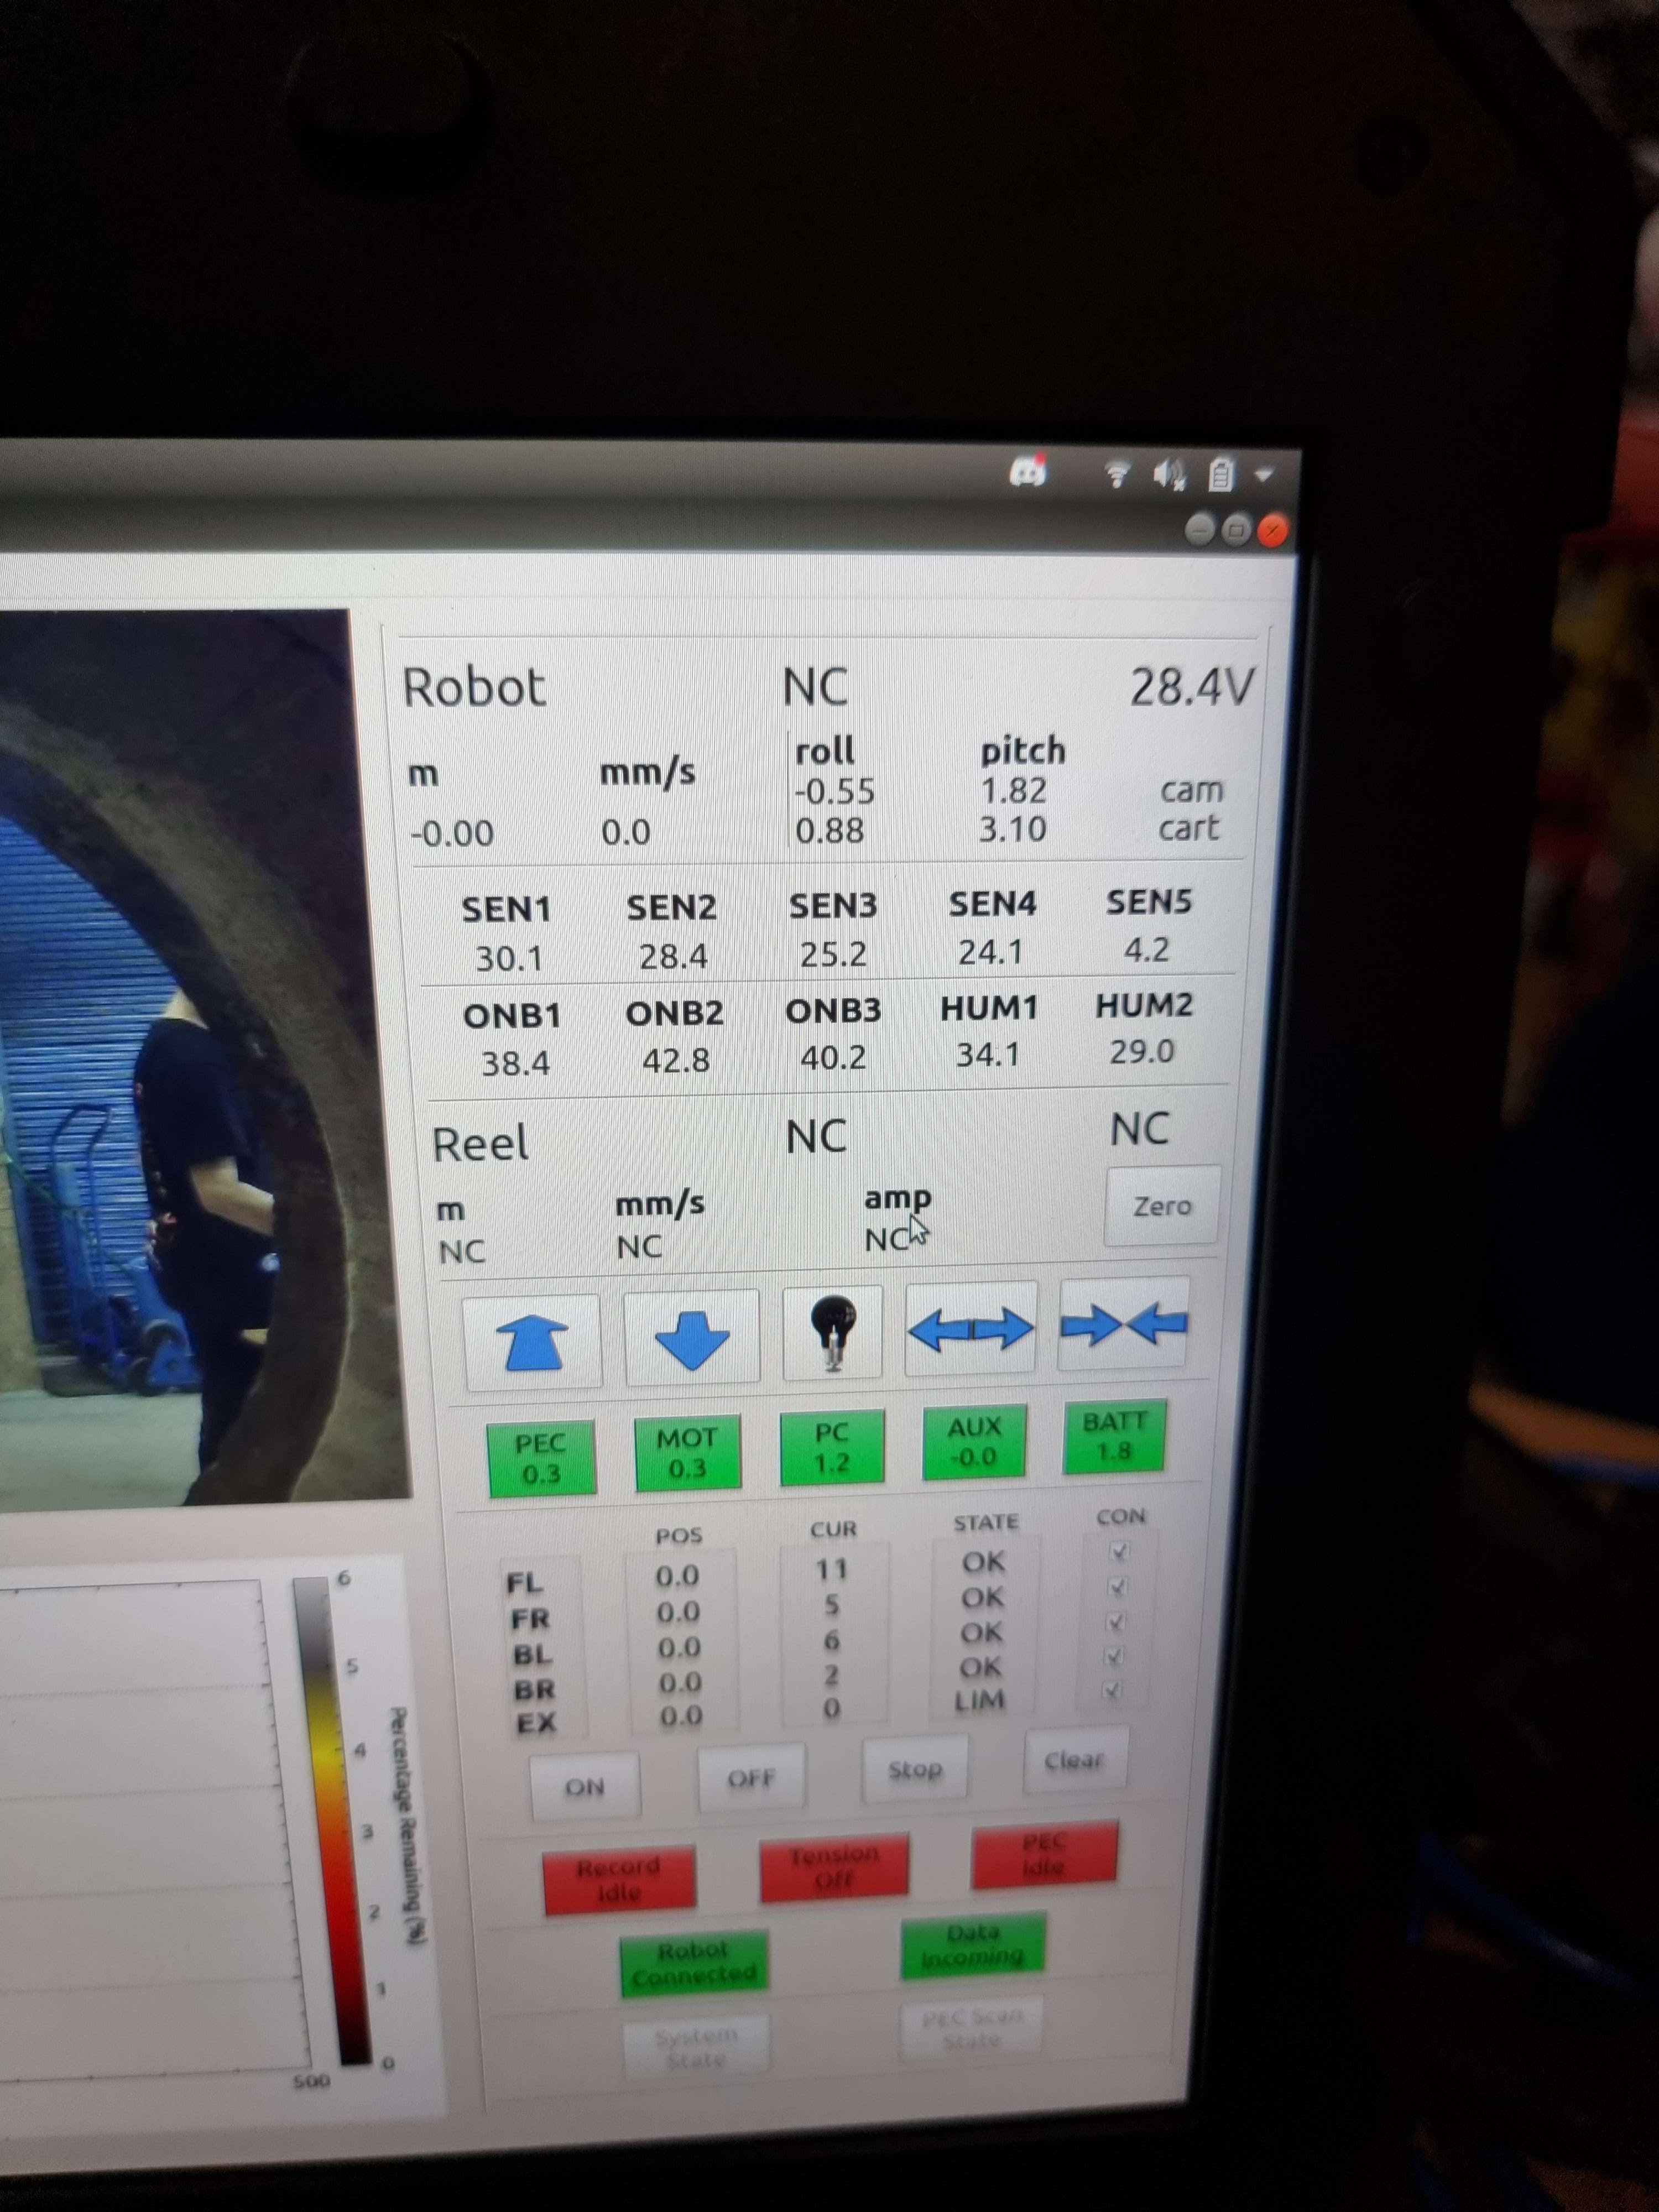
\includegraphics[width=0.30\textwidth, valign=c]{images/rima1/rima1_old_gui.jpg}
    }
    \hspace{0.5cm}
    \subfloat[New RIMA1 interface]{
        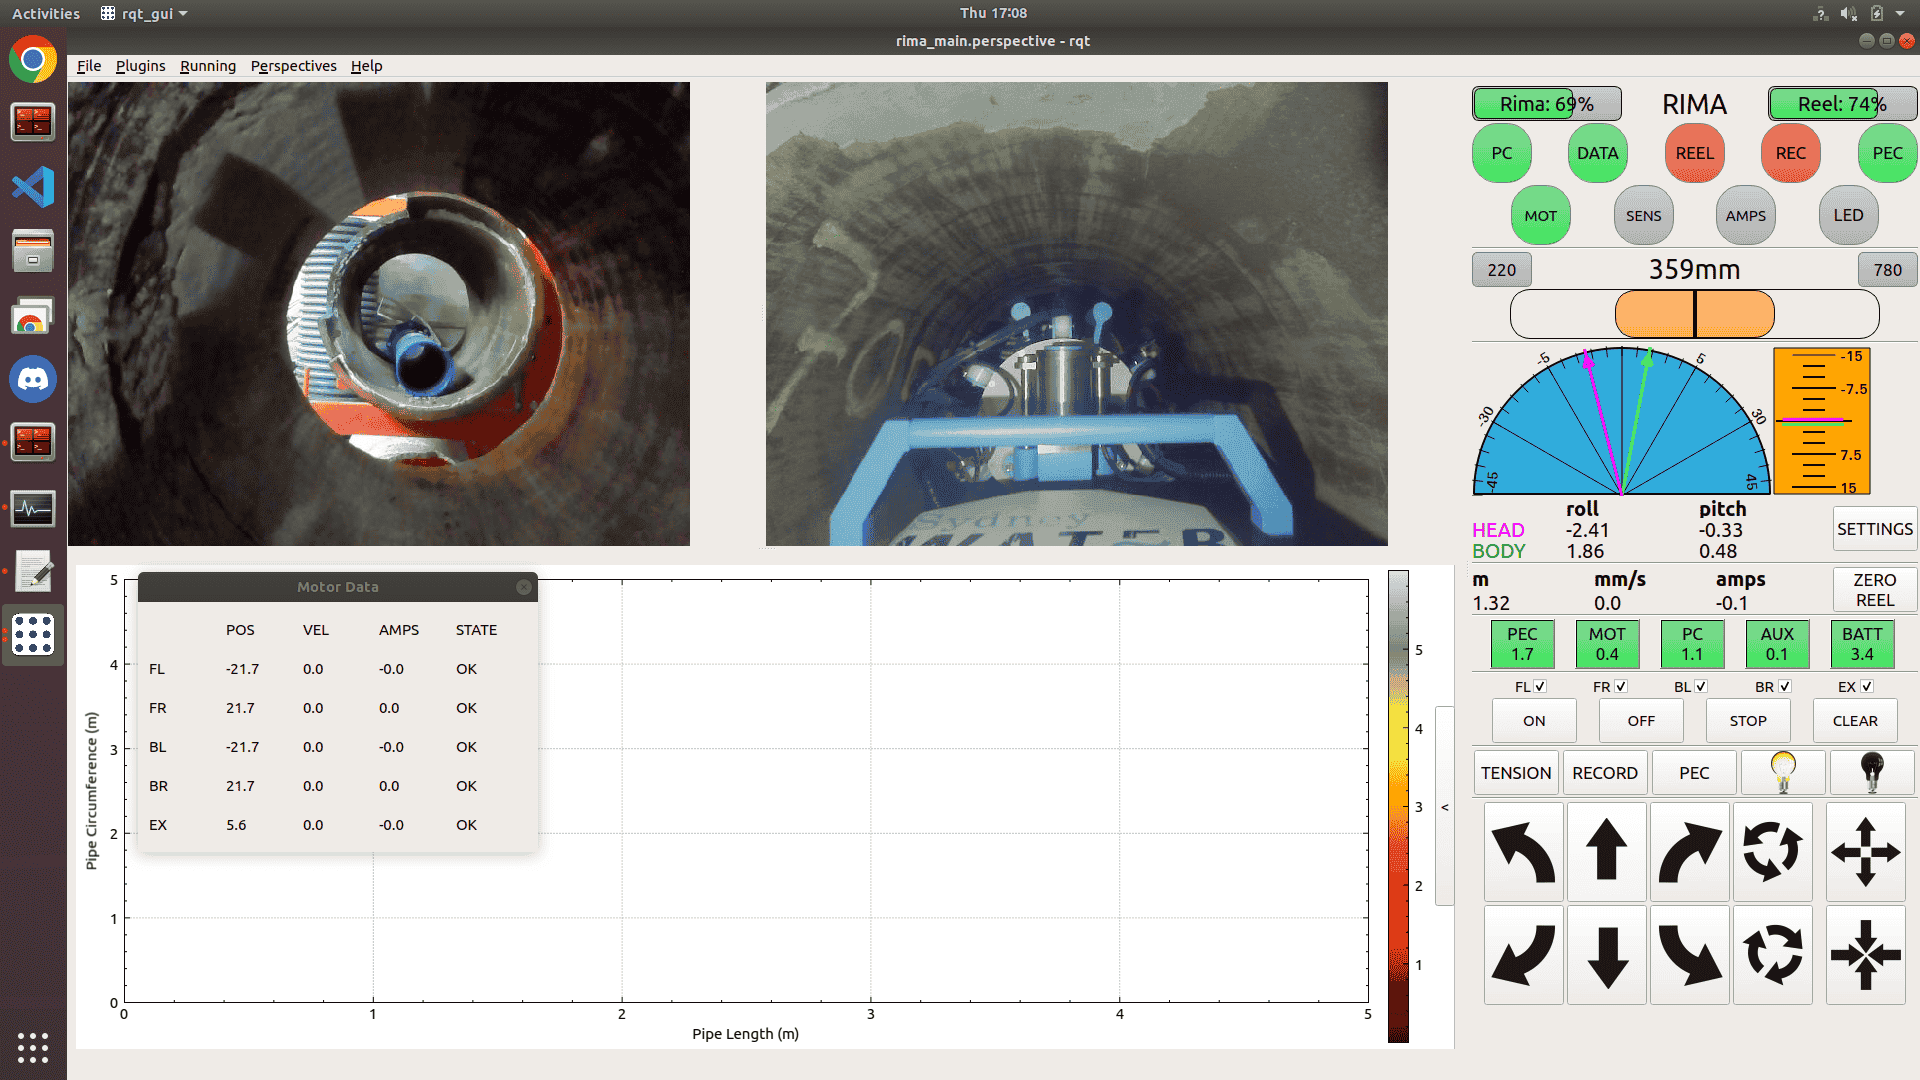
\includegraphics[width=0.60\textwidth, valign=c]{images/rima1/rima_gui_new.png}
    }
    \caption{Comparison of RIMA1 GUI's}
    \label{fig:r1gui}
\end{figure*}
\newpage
\imginin{rima1/rear_cam_rear.jpg}{RIMA1 Rear Camera rear View}{rcam}{0.8}

% Embedded software debugging for RIMA2 PEC

% PEC Calibration

% Simplified shell script for data tranfer
   